\chapter{Experiments}
\label{chap:experiments}
\section{Environment}
We developed our experiments environment cluster were listed as table \ref{talbe:Host}, and created 4 virtual machines in the computer that each of their resource were listed as table \ref{talbe:Virtual Machine}. We will mount NFS to each virtual machines and test 2 types each of NFS, hard disk, and memory(tmpfs). 
In addition, we will test the difference between \textbf{Direct} method that is defined as new checkpoint image and \textbf{Track-memory} method that is defined as pre-dump checkpoint image which is followed by checkpoint images.

\begin{table}[hbtp]
\begin{center}
\begin{tabular}{|c|c|} \hline
CPU & Intel Xeon(R) CPU-E5-2630 v3 @ 2.40GHz x 32 \\ \hline
Memory & 64 GB \\ \hline
Disk & 1.0 TB \\ \hline
OS & Ubuntu 15.10 64 bit \\ \hline
Kernel version & 4.4.4-040404-generic \\ \hline
Docker version & 1.10.3 \\ \hline
Docker Swarm version & 1.2 \\ \hline
Virtual Box version & 5.10.14 \\ \hline
\end{tabular}
\end{center}
\caption{Experiment environment}
\label{talbe:Host}
\end{table}

\begin{table}[hbtp]
\begin{center}
\begin{tabular}{|c|c|} \hline
CPU & Intel Xeon(R) CPU-E5-2630 v3 @ 2.40GHz x 4 \\ \hline
Memory & 8 GB \\ \hline
Disk & 40 GB \\ \hline
OS & Ubuntu 15.10 64 bit \\ \hline
Kernel version & 4.4.4-040404-generic \\ \hline
Docker version & 1.10.3 \\ \hline
Docker Swarm version & 1.2 \\ \hline
\end{tabular}
\end{center}
\caption{Virtual Machine experiment environment}
\label{talbe:Virtual Machine}
\end{table}

\section{Container Migration Time}
As shown in Figure \ref{fig:Docker Swarm migration time with remote storage server}, native is a based line of the other kinds of experiment.
We choose Redis\cite{paksula2010persisting} as our migration container, because it uses memory to save its data. Therefore, we can check the correctness of Redis data to make sure container migration is success.

In the beginning, creating the container on another Swarm Nodes is fast for all environments because we assume that they have downloaded their container images from the remote repository, thus, they do not need to transport container images from the other Swarm Nodes.

Next, in \textbf{Track-memory} method, the container has to pre-dump the checkpoint image at the version-group created. After pre-dumping the checkpoint image, dumping checkpoint will track memory different with the pre-dump checkpoint image.
On the other hand, \textbf{Track-memory} method, checkpoint ticker dumps the checkpoint image directly.
The result of total checkpoint time, \textbf{Track-memory} method is longer than the other one, because it has to add pre-dumping checkpoint time and dumping checkpoint time.
Although \textbf{Track-memory} method is longer, but it provides the less frozen time to the container that improves CPU's utilization.

Third, Restoring the container to the container which has already been created in the Swarm Node. Except NFS with memory, they all have nearly performance.

Final, it has big disparity of the delete checkpoint image step at \textbf{Track-memory} method, because it has more image files and directories than the version without pre-dumping version.

After all, the checkpoint and restoration of container in memory is faster than hard disk in NFS.
As result of Figure \ref{fig:Docker Swarm migration time with remote storage server}, NFS with memory has the best performance in this experiment.

\begin{figure}[hbtp]
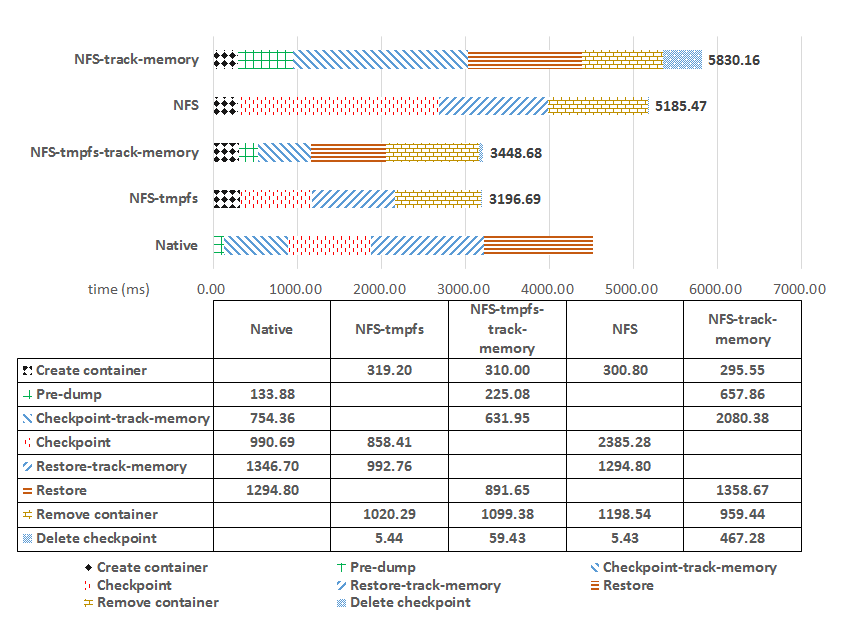
\includegraphics[width=17cm]{figure/migration_time.png}
\caption{Docker Swarm migration with remote storage server}
\label{fig:Docker Swarm migration time with remote storage server}
\end{figure}

\section{The Influence of Container Checkpoint Time on Container Process Time}
\label{sec:CPU Time}
In this experiment, sysbench\cite{kopytov2004sysbench} is used to test performance of process's CPU execution time. Our parameter of sysbench is:
\begin{center}
sysbench --test=cpu --cpu-max-prime=200000 run
\end{center}
It needs to run around 11 minutes in native container without dumping any checkpoint to find the 200000th prime number.

In Figure \ref{fig:Checkpoint Time CPU}, this figure lists every checkpoint time in the experiment environments, also, if remote storage uses the memory to save the checkpoint images, it will get better performance.
In the checkpoint restore rescheduling policy (section \ref{sec:checkpoint restore rescheduling policy}), we set a parameter of checkpoint-ticker period $ T_i $ which will checkpoint repeatedly for every checkpoint-ticker over.

As Figure \ref{fig:Checkpoint Time Influence CPU}, the result of the checkpoint-ticker period $ T_i $ is in direct ratio to the container process execution time.
As these experiment results, the checkpoint-ticker period $ T_i $ has a big influence of container execution time, it is an important parameter in checkpoint restore rescheduling policy that if $ T_i $ is too small, the container will get a bad performance. But if $ T_i $ is too big, whenever Swarm Node fails, the restore container needs to execute the process again. The worst, it might lose some important data. However, no matter the total checkpoint time in \textbf{Track-memory} method, the process's execution time are nearly 
\textbf{Direct} method. This situation shows that the pre-dump checkpoint time has no influence on the process's execution time.

\begin{figure}[hbtp]
\begin{center}
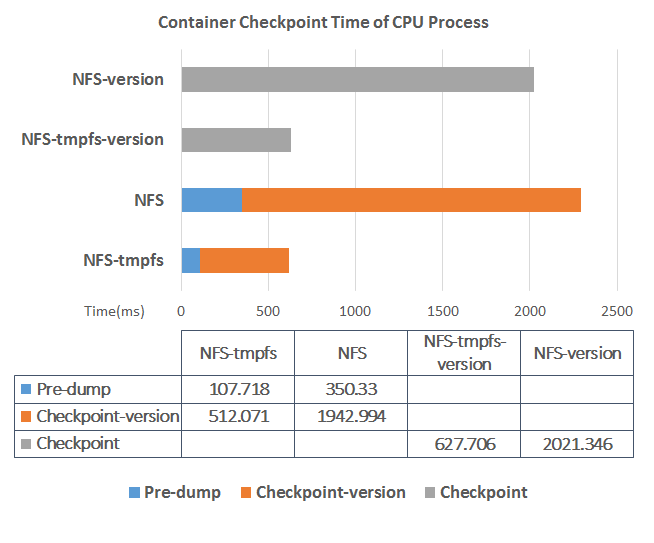
\includegraphics[width=14cm]{figure/cpu_checkpoint_time.png}
\end{center}
\caption{Container checkpoint time of container process time}
\label{fig:Checkpoint Time CPU}
\end{figure}

\begin{figure}[hbtp]
\begin{center}
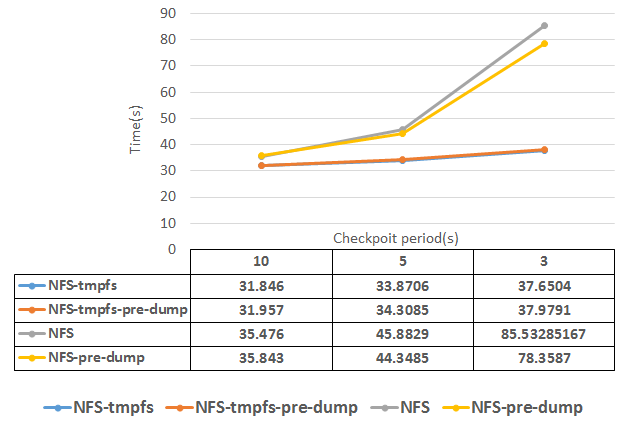
\includegraphics[width=14cm]{figure/cpu_checkpoint_period.png}
\end{center}
\caption{ontainer Checkpoint Time Influence of Container Process Time}
\label{fig:Checkpoint Time Influence CPU}
\end{figure}

\section{The Influence of Container Memory Size on Container Checkpoint Time}
\label{sec:Memory Size}
In this experiment, there are 3 different memory size processes measured. These processes allocate 1 MB, 100 MB, and 1 GB and change the memory with random values quickly in a while loop.

As shown in Figure \ref{fig:1MB}, the pre-dump checkpoint time is at most 1/5 of the checkpoint time and track-memory checkpoint time is about the same as checkpoint time.

However, in Figure \ref{fig:100MB}, the pre-dump checkpoint time is almost a halt of the checkpoint time in the 100 MB process.
In this scenario, the track-memory checkpoint time is still nearly as checkpoint time, but the total checkpoint time is about 1.5 times longer then checkpoint time without track-memory, it means when every version-group is created, the first total checkpoint time is 1.5 times longer then \textbf{Direct} method's checkpoint time .

In the 1 GB process, Figure \ref{fig:1GB} shows that the pre-dump checkpoint time is almost as same as the checkpoint time. It situation shows that the total checkpoint time is about 2 times longer then \textbf{Direct} method when every version-group is created.

In contrast, If the process has allocated the memory but didn't use it, the result will show as Figure \ref{fig:allocate memory}. This figure shows whatever how many memories are allocated in the process, the pre-dump checkpoint time and checkpoint time are all smaller than the process which is allocated memories with changing it.

Follow these experiments, the memory's change has a big influence about container checkpoint time. It is not a effectiveness way when the process need to change memory a lot in the checkpoint-ticker period $ T_i $ time.

\begin{figure}[htbp]
\begin{center}
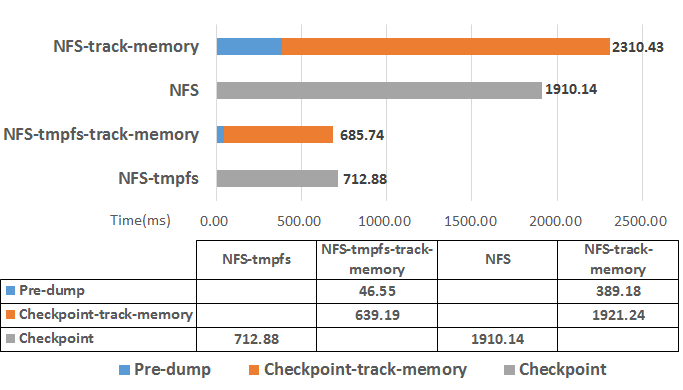
\includegraphics[width=14cm]{figure/1MB.png}
\end{center}
\caption{1MB container process's checkpoint time}
\label{fig:1MB}
\end{figure}

\begin{figure}[htbp]
\begin{center}
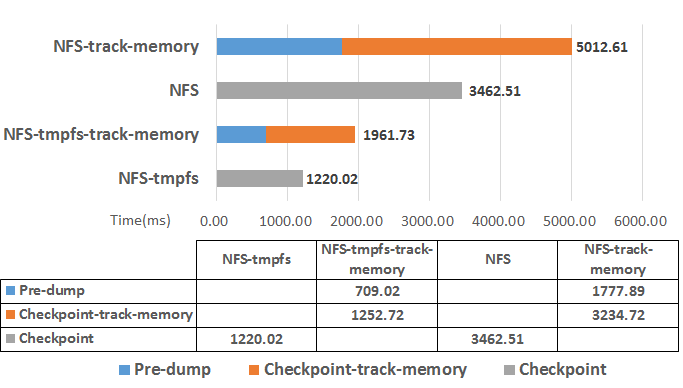
\includegraphics[width=14cm]{figure/100MB.png}
\end{center}
\caption{100MB container process's checkpoint time}
\label{fig:100MB}
\end{figure}

\begin{figure}[htbp]
\begin{center}
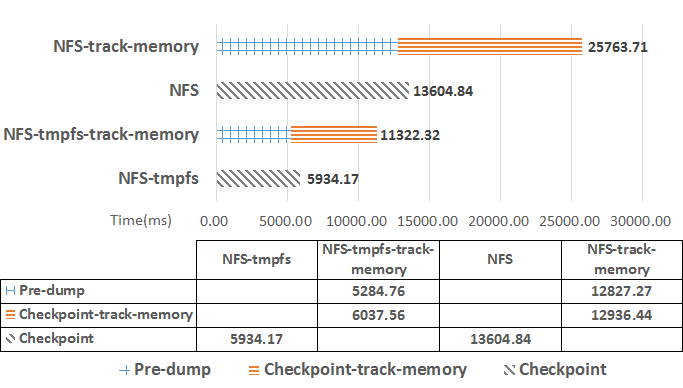
\includegraphics[width=14cm]{figure/1GB.png}
\end{center}
\caption{1GB container process's checkpoint time}
\label{fig:1GB}
\end{figure}

\begin{figure}[htbp]
\begin{center}
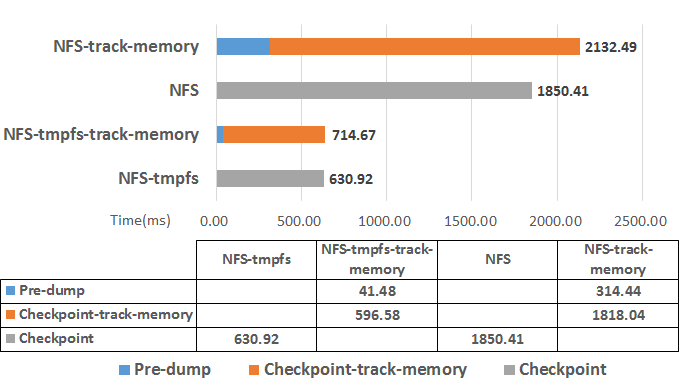
\includegraphics[width=14cm]{figure/allocate_mem_without_change.png}
\end{center}
\caption{Allocated memory without change process's checkpoint time}
\label{fig:allocate memory}
\end{figure}

\section{The Influence of Container Memory Usage on Container Checkpoint Image Size}
In the section \ref{sec:Memory Size}, the container checkpoint time is direct ratio to process memory usage. In this section, the checkpoint images size will be estimated.

In Table \ref{table:process image size}, it shows that the experiments in the section \ref{sec:Memory Size}. If the process uses more memory, the checkpoint image size will be larger. However, although process allocates memory a lot, the checkpoint size still small unless the memory be used.

In Table \ref{table:process image size}, it shows that track-memory version of checkpoint is useless, because it takes more checkpoint time and more storage spaces. To change this view, we test Redis benchmark for daily application. The redis-benchmark command is:
\begin{center}
redis-benchmark -t set -l
\end{center}
This command will send 100000 requests with 50 parallel clients. The results shown as table \ref{table:redis image size}, the pre-dump checkpoint image size is similar as checkpoint image size, but the track-memory checkpoint image size is smaller than the others. This experiment result shows that the Table \ref{table:process image size} is the worst case in checkpoint image size. In this case, if track-memory checkpoint is used, it will save more than 2 times storage space.

As these results, we observe the container checkpoint image size is related with the container checkpoint time.
When the container checkpoint time increasing, the container checkpoint image size will increase, too.
When the container checkpoint image size over 500 MB, it means that the container memory has changed a lot, pre-dump checkpoint is an inefficient action.
To avoid unnecessary container pre-dump, whenever container checkpoint group's average image size over 500 MB, next checkpoint group will not pre-dump the container checkpoint.

\begin{table}[hbtp]
\begin{center}
\begin{tabular}{|c|c|c|c|c|}\hline 
• & 1 MB & 100 MB & 1 GB & Allocate memory without changing\\ 
\hline 
Pre-dump & 1 MB & 100 MB & 1 GB & 102 KB\\ 
\hline 
Checkpoint-track-memory & 1 MB & 100 MB & 1 GB & 90.9 KB \\ 
\hline 
Checkpoint & 1 MB & 100 MB & 1 GB & 175.2 KB \\ 
\hline 
\end{tabular}
\caption{Process allocated memory's checkpoint image size}
\label{table:process image size}
\end{center}
\end{table}

\begin{table}[hbtp]
\begin{center}
\begin{tabular}{|c|c|c|}
\hline 
• & Redis & Redis-benchmark \\ 
\hline 
Pre-dump & 9 MB & 14 MB \\ 
\hline 
Checkpoint-track-memory & 2.3 MB & 2.3 MB \\ 
\hline 
Checkpoint & 9.6 MB & 14 MB \\ 
\hline 
\end{tabular}
\caption{Redis and Redis benchmark's checkpoint image size}
\label{table:redis image size}
\end{center}
\end{table}

\section{The Influence of Many Containers Checkpoint in The Same Time on Container Checkpoint Time}
Figure \ref{fig:many containers} demonstrates the influence of checkpoint time when many containers checkpoint in the same.
As more containers checkpoint in the same time, the more checkpoint time for each container has to take.
In storing in disk case, it almost needs twice times when 4 containers checkpointing in the same time. That's the reason that we implement checkpoint queue to solve this problem.

\begin{figure}[htbp]
\begin{center}
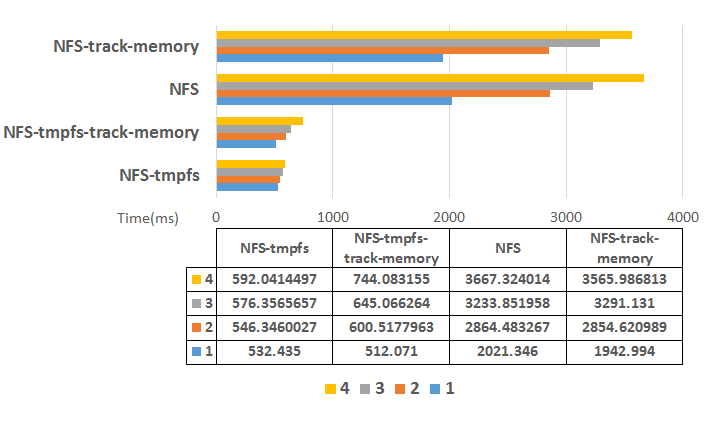
\includegraphics[width=14cm]{figure/many_containers.png}
\end{center}
\caption{Many containers checkpoint in the same time}
\label{fig:many containers}
\end{figure}

\section{The Influence of Container Checkpoint Versions on Container Checkpoint Time}
As Figure \ref{fig:versions}, \textbf{Direct} method's checkpoint time average have 2 horizontal lines.
Two \textbf{Track-memory} method's trendline are slow increasing when the container checkpoint versions growing up.
Each of them has one point of intersections with \textbf{Direct} method's checkpoint time line, the values are and 5 and 16.
Follow these results, checkpoint-version default value sets to 5 is a better choice, and it should not exceed than 16.

\begin{figure}[htbp]
\begin{center}
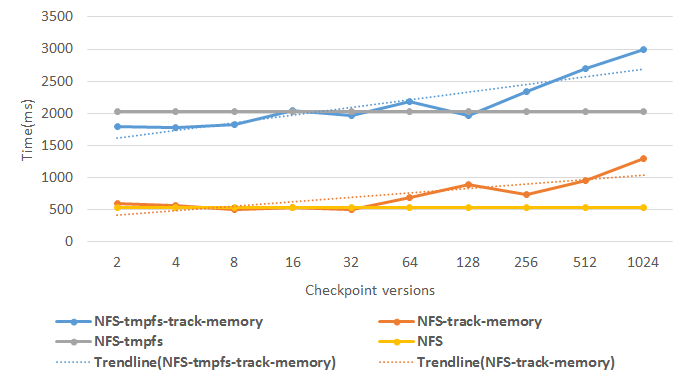
\includegraphics[width=14cm]{figure/versions.png}
\end{center}
\caption{Checkpoint versions of container checkpoint time}
\label{fig:versions}
\end{figure}
